\chapter{The Universe in a Computer}

\section{Gravity}

Gravity is the weakest of all fundamental forces in physics, far
weaker than electromagnetism or the so-called weak and strong
interactions between subatomic particles.  However, the other three
forces lose out in the competition with gravity over long distances.
The weak and strong interactions both have an intrinsically short
range.  Electromagnetism, while being long-range like gravity, suffers
from a cancellation of attraction and repulsion in bulk matter, since
there tend to be as almost exactly as many positive as negative
charges in any sizable piece of matter.  In contrast, gravitational
interactions between particles are always attractive.  Therefore, the
larger a piece of matter is, the more gravitational force it exerts on
its surroundings.

This dominance of gravity at long distances makes the job of
modeling a chunk of the Universe easier.  To a first approximation, it
is often a good idea to neglect the other forces, and to model the
objects as if they were interacting only through gravity.  In many
cases, we can also neglect the intrinsic dimensions of the objects,
treating each object as a point in space with a given mass.  All this
greatly simplifies the mathematical treatment of a system, by leaving
out most of the physics and chemistry that would be needed in a more
accurate treatment.

This book is the first in a series of books titled {\it Pure Gravity}, to
indicate that we are making this approximation of treating objects as
gravitating masses and nothing more.  The objects we will be studying
are stars, and the environment we will focus on are dense stellar
systems, where the stars are so close together that they will
occasional collide and in general have frequent interesting and
complex interactions.  In a later series, {\it Applied Gravity}, we will
look at the internal physics of those stars: how they evolve under the
influence of nuclear reactions in their centers, how they may die in
cosmic explosions, and what happens to their remnant cores.  We will
especially study how interactions between stars of all types can change
their evolutionary behavior through two-body, three-body, and more
complex interactions, leading to an intricate `star cluster ecology'.

This first book, {\it Writing an N-Body Code}, lays the groundwork for
modeling a system of stars.  We start absolutely from scratch, with a
most simple code of less than a page long.  In many small steps we
then improve that code, pointing out the many pitfalls along the way,
on the level of programming as well as astrophysical understanding.
We introduce helpful code development facilities and give many hints as
to how to balance simplicity, efficiency, clarity, and modularity of
the code.  Our intention is to introduce the topic from square one,
and then to work our way up to a robust set of codes with which one
can do actual research.  In later volumes in this series, we will
continue to develop these codes, adding many useful diagnostic tools,
and integrating those in a full production-level software environment.

\section{Galactic Suburbia}

The sun is a star like any other among the hundred billion or so stars
in our galaxy.  It is unremarkable in its properties.  Its mass is in
the mid range of what is normal for stars: there are others more than
ten times more massive, and there are also stars more ten times less
massive, but the vast majority of stars have a mass within a factor
ten of that of the sun.  Our home star is also unremarkable in its
location, at a distance of some thirty thousand light years from the
center of the galaxy.  Again, the number of stars closer to the center
and further away from the center are comparable.  Our closest neighbor,
Proxima Centauri, lies at a distance of a bit more than four light years.

This distance is typical for separations between stars in our neck of
the woods.  A light year is ten million times larger than the diameter
of the sun (a million km, or three light seconds).  In a scale model,
if we would represent each star as a cherry, an inch across, the
separation between the stars would be many hundreds of miles.  It is
clear from these numbers that collisions between stars in the solar
neighborhood must be very rare.  Although the stars follow random
orbits without any traffic control, they present such tiny targets
that we have to wait very long indeed in order to witness two of them
crashing into each other.  A quick estimate tells us that the sun has
a chance of hitting another star of less than $10^{-18}$ per year.  In
other words, we would have to wait at least $10^{18}$ years to have an
appreciable chance to witness such a collision.  Given that the sun is
less than five billion years old, it is no surprise that it does not
show any signs of a past collision: the chance that that would have
happened was less than one in a hundred million.  Life in our galactic
suburbs is really quite safe for a star.

There are other places in our galaxy that are far more crowded, and
consequently are a lot more dangerous to venture into.  We will have
a brief look at four types of crowded neighborhoods.

\section{Globular Clusters}

\begin{figure}[ht]
\centering
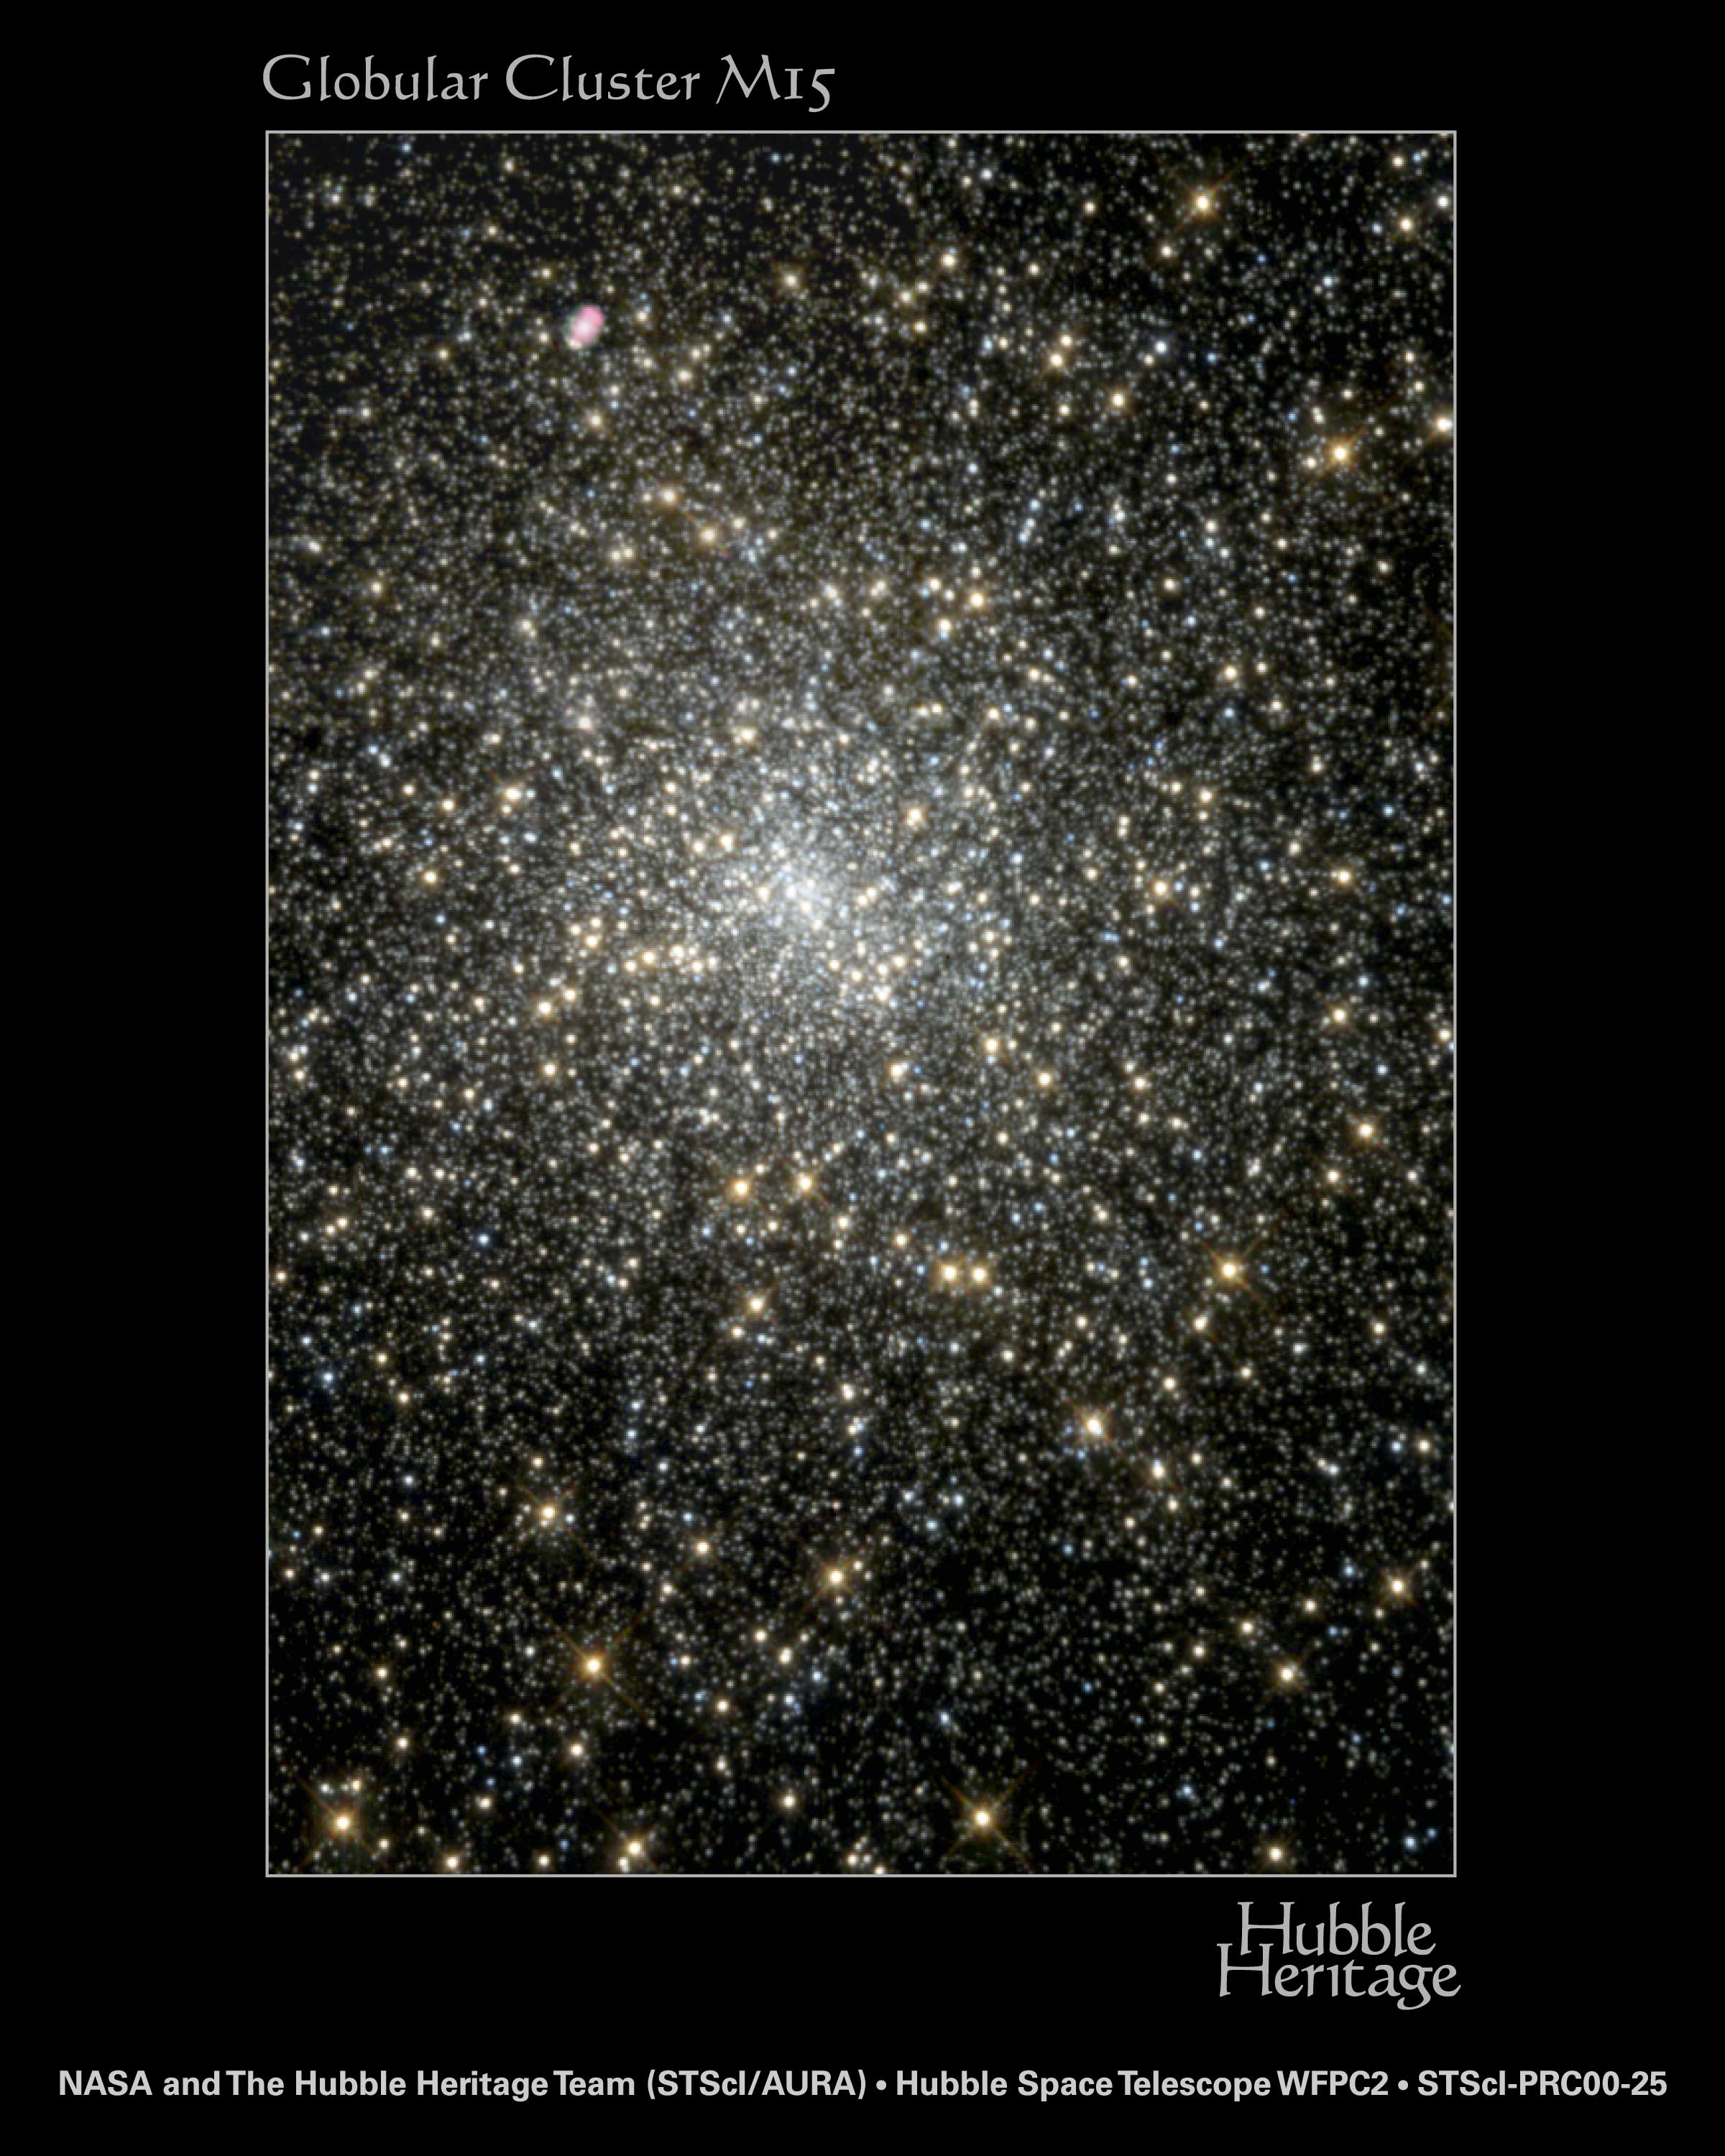
\includegraphics[width=4.5in]{chap1/m15.eps}
\caption[A snapshot of the globular cluster M15]
{A snapshot of the globular cluster M15, taken with the Hubble Space
Telescope.}
\label{fig:m15}
\end{figure}
%%  From: http://oposite.stsci.edu/pubinfo/PR/2000/25/content/0025y.jpg

In Fig. \ref{fig:m15} we see a picture of the globular cluster M15,
taken with the Hubble Space Telescope.  This cluster contains roughly
a million stars.  In the central region typical distances between
neighboring stars are only a few hundredth of a light year, more than
a hundred times smaller than those in the solar neighborhood.  This
implies a stellar density that is more than a million times larger
than that near the sun.  Since the typical relative velocities of
stars in M15 are comparable to that of the sun and its neighbors, a
few tens of km/sec, collision times scale with the density, leading to
a central time between collisions of less than $10^{12}$ years.  With
globular clusters having an age of more than $10^{10}$ years, a typical
star near the center already has a chance of more than a percent to
have undergone a collision in the past.  

In fact, the chances are much higher than this rough estimate indicates.
One reason is the stars spend some part of their life time in a much
more extended state.  A star like the sun increases its diameter by
more than a factor of one hundred toward the end of its life, when
they become a red giant.  By presenting a much larger target to other
stars, they increase their chance for a collision during this stage
(even though this increase is partly offset by the fact that the red
giant stage lasts shorter than the so-called main-sequence life time
of a star, during which they have a normal appearance and diameter).
The other reason is that many stars are part of a double star system,
a type of dynamic spider web that can catch a third star, or another
double star, into a temporary three- or four-body dance.  Once engaged
in such a dance, the local stellar crowding is enormously enhanced,
and the chance for collisions is greatly increased. 

A detailed analysis of all these factors predicts that a significant
fraction of stars in the core of a dense globular cluster such as M15
has already undergone at least one collision in its life time.  This
analysis, however, is quiet complex.  To study all of the important
channels through which collisions may occur, we have to analyze
encounters between a great variety of single and double stars, and
occasional bound triples and larger bound multiples of stars.  Since
each star in a bound subsystem can be a normal main-sequence star, a
red giant, a white dwarf, a neutron star or even a black hole, as well
as an exotic collision product itself, the combinatorial richness of
flavors of double stars and triples is enormous.  If we want to pick a
particular double star, we not only have to choose a star type for
each of its members, but in addition we have to specify the mass of
each star, and the parameters of its orbit, such as the semimajor axis
(a measure for the typical separation of the two stars) as well as the
orbital eccentricity.

The goal of our book series is to develop the software tools to make
it possible to simulate an entire star cluster like M15, and to
analyze the resulting behavior both locally and globally.

\clearpage  % to let the m15 picture be inserted not further than here

\section{Galactic Nuclei}

In Fig. \ref{fig:gc} we see an image of the very center of our galaxy.
This picture is taken with the Northern branch of the two Gemini
telescopes, which is located in Hawaii on top of the mountain Mauna Kea.

\begin{figure}[ht]
\centering
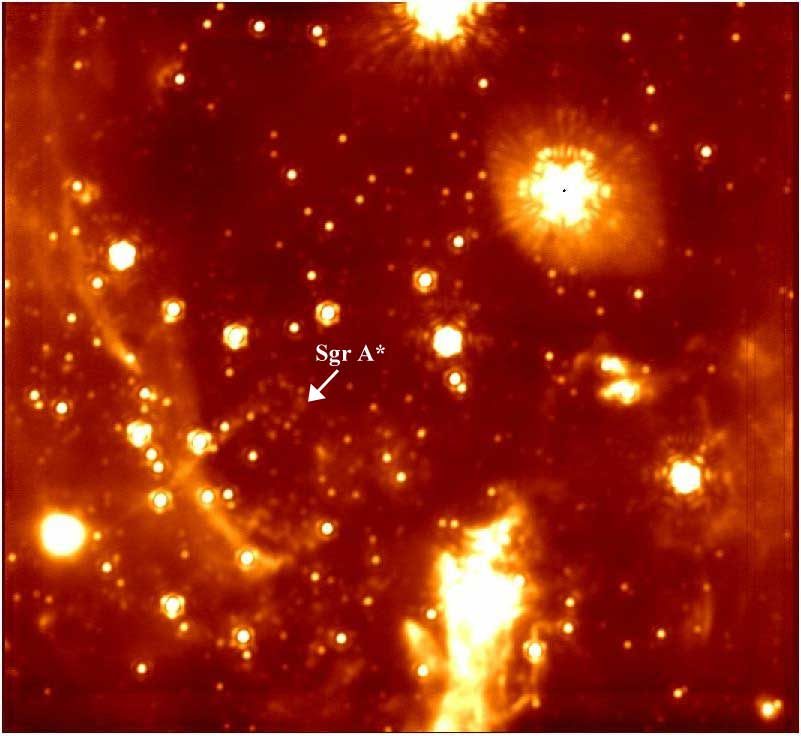
\includegraphics[width=4.5in]{chap1/gc.eps}
\caption[An image of the central region of our galaxy]
{An image of the central region of our galaxy, taken with the Gemini
North telescope.  The center is located on the right just above the
bottom edge of the image.}
\label{fig:gc}
\end{figure}
%% From: http://www.gemini.edu/gallery/observing/gc\_color.jpg

In the very center of our galaxy, a black hole resides with a mass
a few million times larger than the mass of our sun.  Although the
black hole itself is invisible, we can infer its presence by its
strong gravitational field, which in turn is reflected in the speed
with which stars pass near the black hole.  In normal visible light it
is impossible to get a glimpse of the galactic center, because of the
obscuring gas clouds that are positioned between us and the center.
Infrared light, however, can penetrate deeper in dusty regions.
Fig. \ref{fig:gc} is a false-color image, reconstructed from
observations in different infrared wavelength bands.

In the central few light years near the black hole, the total mass of
stars is comparable to the mass of the hole.  This region is also
called the galactic nucleus.  Here the stellar density is at least as
large as that in the center of the densest globular clusters.  However,
due to the strong attraction of the black hole, the stars zip around at
much higher velocities.  Whereas a typical star in the core of M15 has
a speed of a few tens of km/sec, stars near the black hole in the
center of our galaxy move with speeds exceeding a 1000 km/sec.  As a
consequence, the frequency of stellar collisions is strongly enhanced.

Modeling the detailed behavior of stars in this region remains a great
challenge, partly because of the complicated environmental features.
A globular cluster forms a theorist's dream of a laboratory, with its
absence of gas and dust and starforming regions.  All we find there
are stars that can be modeled well as point particles unless they come
close and collide, after which we can apply the point particle
approximation once again.  In contrast, there are giant molecular
clouds containing enormous amounts of gas and dust right close up to
the galactic center.  In these clouds, new stars are formed, some of
which will soon afterwards end their life in brilliant supernova
explosions, while spewing much of their debris back into the
interstellar medium.  Such complications are not present in globular
clusters, where supernovae no longer occur since the member stars are
too old and small to become a supernova.

Most other galaxies also harbor a massive black hole in their nuclei.
Some of those have a mass of hundreds of millions of solar masses, or
in extreme cases even more than a billion times the mass of the sun.
The holy grail of the study of dense stellar systems is to perform and
analyze accurate simulations of the complex ecology of stars and gas
in the environment of such enormous holes in space.  Much of the
research on globular clusters can be seen as providing the initial
steps toward a detailed modeling of galactic nuclei.

\section{Star Forming Regions}

\begin{figure}[ht]
\centering
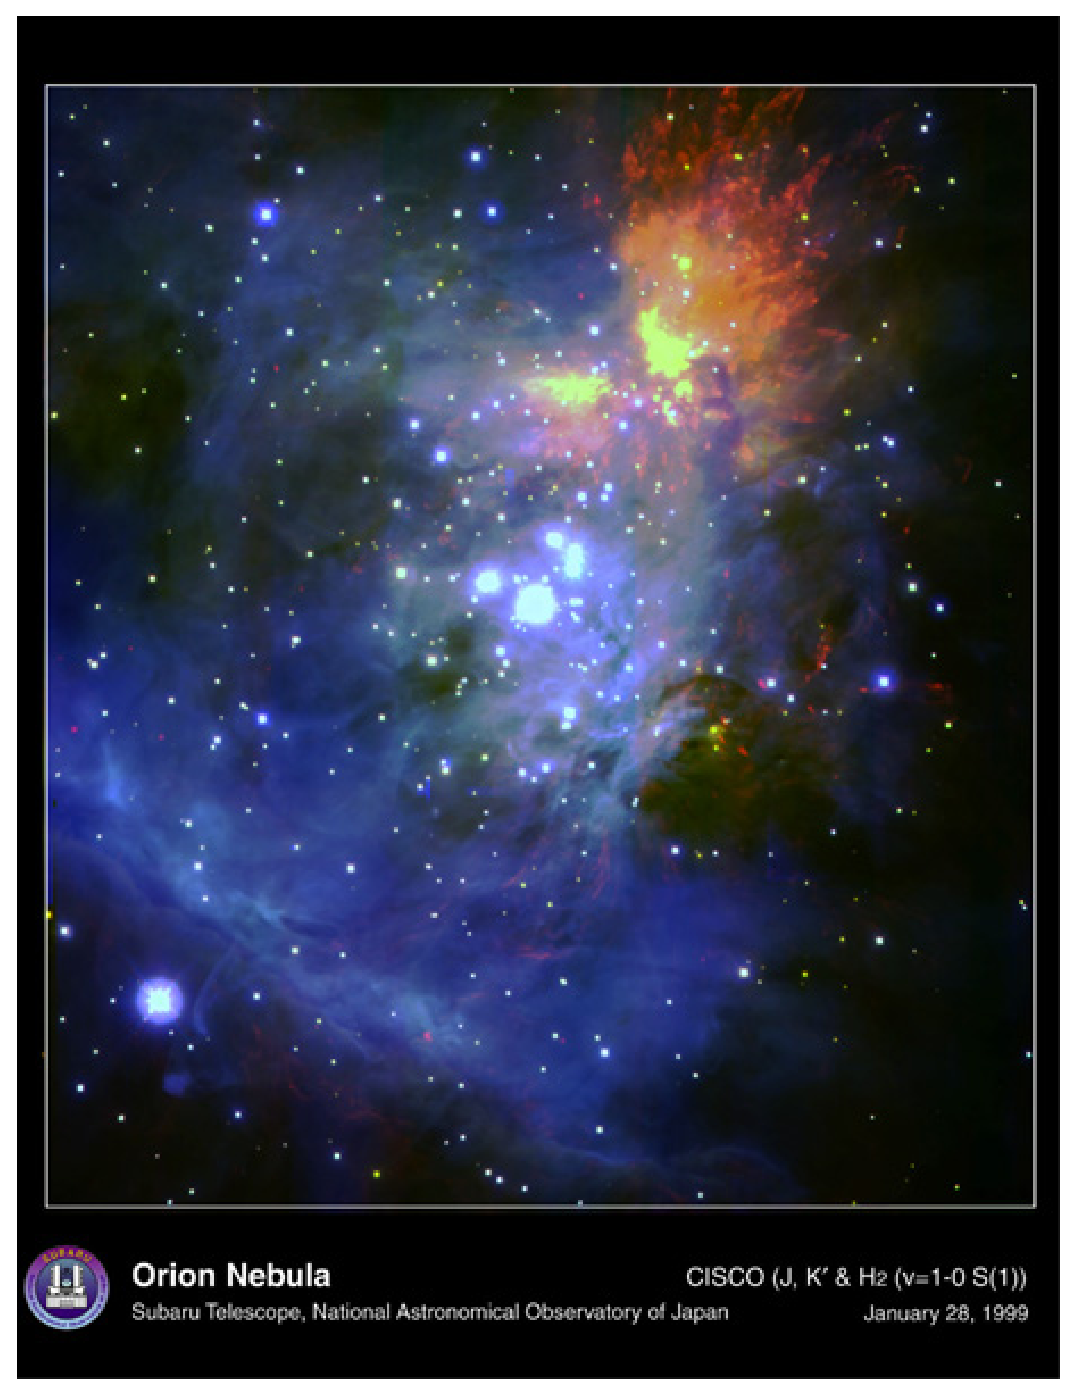
\includegraphics[width=3in]{chap1/orion.eps}
\caption[The Orion Nebula]
{The Orion Nebula, as seen by the Subaru telescope.}
\label{fig:orion}
\end{figure}
%%  From: http://www.subaru.naoj.org/Science/press\_release/9901/Orion.jpg

There are many other places in the galactic disk where the density of
stars is high enough to make collisions likely, at least temporarily.
These are the sites where stars are born.  Fig. \ref{fig:orion} taken
by the Japanese Subaru telescope in Hawaii shows the Orion Nebula,
also known as M42, at a distance of 1500 light years from the sun.
This picture, too, is taking in infrared light in order to penetrate
the dusty regions surrounding the young stars.  The four brightest
stars in the center, collectively known as the Trapezium, form the
most massive stars of a larger conglomeration of stars, all recently
formed from the gas and dust that still surrounds them.

In order to study collisions in these star forming regions, we can no
longer treat the stars are point masses.  Many of the collisions take
place while the stars are still in the process of forming.  While a
protostar is still in the process of contracting from the gas cloud
in which it was born, it presents a larger target for collisions with
other stars.  In addition, a single contracting gas cloud may fission,
giving rise to more than one star at the same time.  In this way, the
correlated appearance of protostars is even more likely to lead to
subsequent collisions.

The proper way to model these processes is to combine gas dynamics and
stellar dynamics.  Much progress has been made recently in this area.
One way to use stellar dynamics in an approximate fashion is to begin
with the output of the gas dynamics codes, which present the positions
and velocities of a group of newly formed stars, and then to follow
and analyze the motions of those stars, including their collisions.

\section{Open Clusters}

Although stars are formed in groups, these groups typically do not
stay together for very long.  Perturbations from other stars and gas
clouds in their vicinity are often enough to break up the fragile
gravitational hold they initial have over each other.  Some of the
more massive groups of newly formed stars, however, are sufficiently
tightly bound to survive their environmental harassment.  They form
the so-called open clusters, where there name indicates that they have
central densities that are typically less than what we see in globular
clusters.

\begin{figure}[ht]
\centering
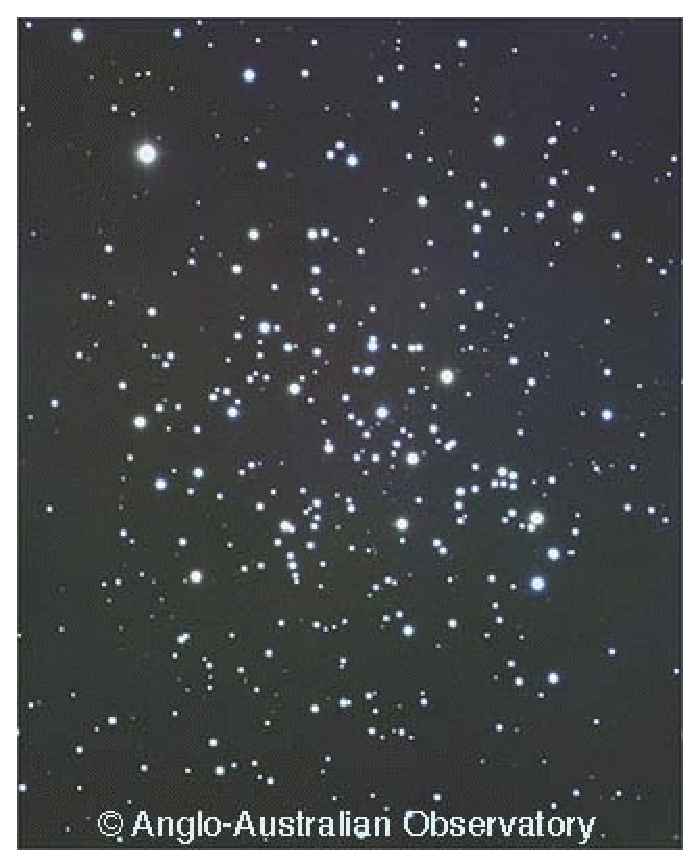
\includegraphics[width=2.5in]{chap1/m67.ps}
\caption[The open star cluster M67]
{The open star cluster M67, in a picture taken by the Anglo-Australian
Observatory.}
\label{fig:m67}
\end{figure}
%%  From: http://www.seds.org/messier/Pics/More/m67aat.jpg

Fig. \ref{fig:m67} shows one of the richest and densest open clusters,
M67, as observed by the Anglo-Australian Observatory.  Since this
cluster is old enough to have lost its gas and dust, all stars are
visible at normal optical wavelengths, at which this image is taken.
In the central regions of this cluster, there are indications that
some of the stars have undergone close encounters or even collisions.
Consequently, this star cluster qualifies as a dense stellar system.

Open clusters typically have fewer members than globular clusters.
Also, they are younger.  Both facts makes it easier to simulate open
clusters than globular clusters.  On the other hand, the densest
globular clusters show a higher frequency and a far richer variety of
stellar collisions, making them a more interesting laboratory.  In
that sense, a dynamical simulation of an open cluster can be seen as
providing preparatory steps toward the modeling of globular clusters,
just as a study of the latter forms a stepping stone toward the
investigation of galactic nuclei.

\section{Writing your own star cluster simulator}

Astronomers have almost half a century of experience in writing
computer codes to simulate dense stellar systems.  The first published
results date back to 1960, and it was in the subsequent decade that it
became clear just how tricky it was to simulate a group of interacting
stars.  The task seems so easy: just integrate Newton's equations of
motion for each star, under the influence of the gravitational pairwise
interactions of all other stars.  Indeed, it is straightforward to
write a simple code to do so, as we will see below.  And as long as
all stars remain fairly well separated from each other, even a simple
code will do a reasonably good job.

In practice, though, even a small group of stars will spontaneously
form one or more double stars.  This was discovered experimentally in
the early sixties.  One way to understand this result, after the fact,
is from an energetic point of view.  When a double star, or binary as they
are generally called, is formed, energy is released.  Since the two stars
in a binary are bound, the potential energy is larger than the kinetic
energy, and the total energy is negative.  When three stars come together
randomly, there is a chance that two of the three are left in a bound
state, while the third one escapes, carrying the excess energy.  Left
by itself, a stellar system will exploit this energy liberation
mechanism by spontaneously forming binaries.

As soon as even one binary appears, a simple code with constant time
steps will either crash or resort to a very slow and inefficient crawl.
The changes in the relative configuration of the two stars occur so
frequent that they can be easily missed.  If they are modeled correctly,
by choosing a tiny time step, the rest of the system will be forced to
slow down, while spending a large and unnecessary amount of computer
time on all the other stars that don't need such fine resolution.  By
the end of the sixties, these problems were overcome by the development
of codes that employed individual time steps.  Stars with close
neighbors were stepped forward in time more frequently than stars at
large, and in this way the computational power was brought to where it
was most needed.

This modification in itself brought gravitational $N$-body codes already
well outside the range of systems that are normally discussed in text
books on numerical integration methods.  The internal book keeping
needed to write a correct and efficient code with individual time
steps is surprisingly large, given the simplicity of the task:
integrate the effect of pairwise attractive inverse square forces.
But this was only a first step toward the development of modern $N$-body
codes.  The presence of tight binaries produced much more of an obstacle,
and throughout the seventies a variety of clever mechanisms were developed
in order to deal with them efficiently.

For one thing, there are problems with round-off.  Two stars in a tight
orbit around each other have almost the same position vector, as seen
from the center of a star cluster, where we normally anchor the global
coordinate system.  And yet it is the separation between the stars
that determines their mutual forces.  When we compute the separation
by subtracting two almost identical spatial vectors, we are asking for
(numerical) trouble.  The solution is to introduce a local coordinate
system whenever two or more stars undergo a close interaction.  This
does away with the round-off problem, but it introduces a host of
administrative complexities, in order to make sure that any arbitrary
configuration of stars is locally presented correctly -- and that the
right thing happens when two or more of such local coordinate patches
encounter each other.  This may not happen often, but one occurrence
in a long run is enough to crash the system if no precautions have
been taken for such a situation to happen.

We can continue the list of tricks that have been invented to allow
every larger and denser systems to be modeled correctly.  Numerical
problems with the singularity in the two-body system have been
overcome by mapping two or more interacting stars from the
three-dimensional Kepler problem to a four-dimensional harmonic
oscillator.  The total force on particles has been split into
different contributions, the first from a near zone of relatively
close neighbors and the second from a far zone of all other particles,
with each partial force being governed with different integration time
steps.  Tree codes have been used to group the contributions of a
number of more and more distant zones together in ever larger chunks,
for efficiency.  Triple stars have received their own special treatment,
especially the marginally stable triples that are sometimes long-lived, 
but continuously changed their inner state due to internal perturbations.
The list goes on.

In this first book, we will introduce a modern integrator, the Hermite
scheme, developed in the 1990s, together with a variable time step
integration scheme, where all stars share a common time step at any
given time.  In subsequent volumes in the series, we will introduce
the other refinements mentioned above.  Our emphasis will be on a
complete explanation of all the steps involved, together with a
discussion of the motivation for those steps.  In the last few
chapters, we will embark on a research project featuring stellar
collisions, in a simple gravity-only approximation.
